\chapter{Screen-based semantic speech editing}\label{sec:screen}

In Chapter~\ref{sec:ethno}, the radio producers we observed all used textual representations to navigate and edit audio
content. The drama producers used a script to write notes on what they recorded, any changes or mistakes that were made, and the
quality of the performances. The documentary producers wrote transcripts of their recordings to help them navigate and
arrange their content, and to mark up the parts they wanted to use in the programme. The news journalists also used
text to label their audio clips with the words spoken at the start and end of the clip.

In Section~\ref{sec:background-transcripts} we saw that transcripts have been successfully used to develop interfaces
that allow for semantic navigation and editing of speech content.  \citet{Whittaker2002} found that their semantic
speech interface could be used to quickly extract information and judge which parts were relevant, without having to
play the audio.  \citet{Whittaker2004} found that semantic editing was faster and as accurate as editing with a
waveform-based interface, and \citet{Sivaraman2016} found that semantic editing was more accessible than waveform
editing.  \citet{Rubin2013} presented a semantic speech interface for producing ``audio stories'', which has many
similarities to radio production. However, this system was not formally tested, so it is still unclear what effect
semantic editing interfaces have on the production of audio content.

We saw in Chapter~\ref{sec:ethno} that the documentary producers we observed either manually transcribed their
recordings, which may not be the best use of their time, or paid a third-party to transcribe on their behalf, which is
slow and expensive.  As we discussed in Section~\ref{sec:asr}, automatic speech recognition (ASR) could be used to
replace the manual transcription process. However, the errors in ASR transcripts reduce listener comprehension
\citep{Stark2000,Vemuri2004} and increase the time it takes to search audio content \citep{Ranjan2006} and correct
errors \citep{Burke2006}. The semantic speech editor from \citet{Rubin2013} used verbatim transcripts, so it is not
clear how these errors might affect audio production. Several semantic speech editors that used ASR were formally
evaluated \citep{Whittaker2004,Yoon2014,Sivaraman2016}, but they were designed for navigating and editing voice
messages and comments, which use a different style of audio content and have different requirements than radio
production.










We were interested in investigating whether semantic speech editing can be used for radio production, and understanding
what effect semantic editing and ASR transcripts have on the production process.  In this chapter, we describe the
design and development of \textit{Dialogger} -- a semantic speech editing interface for radio production, and explain
how we evaluated our system with radio producers at the BBC.

In Section~\ref{sec:screen-requirements}, we review the existing production process to gather requirements for the
design of our system.  In Section~\ref{sec:screen-design}, we describe the design and development of Dialogger.  In
Section~\ref{sec:screen-methods}, we outline the methodology of our contextual user study in which radio producers used
Dialogger as part of the production of real radio programmes. We present the results of our study in
Section~\ref{sec:screen-results}, discuss our findings and their implications in Section~\ref{sec:screen-discussion}
and present our conclusions in Section~\ref{sec:screen-conclusion}.















\section{System requirements}\label{sec:screen-requirements}


In this section, we will review the results of our study in Chapter~\ref{sec:ethno} and map our observations into
system requirements for our semantic editing system.

We saw that the producers of the documentary ``logged'' each interview they recorded by transcribing it themselves, or
by paying a third-party service to write a full transcription.  They then used the transcripts to select which bits
they wanted to use, and copied the text to create a rough script of the programme. Once the script was mostly complete,
they had to find and cut each piece of audio for the programme, then assemble them into a draft composition known as a
``rough edit''.

Both the transcription and rough edit processes are time-consuming for the producer. Semantic speech
editing may be able to make these two production activities more efficient. We will consider these
individually to gather high-level requirements for our system.

\subsection{Transcription}
As we discovered in Chapter~\ref{sec:ethno}, radio programmes are assigned a slot in the broadcast schedule, so
producers have a strict deadline for finishing their programme. Programmes are sometimes scheduled up to three
weeks in advance, but sometimes as little as one week in advance.  This means that producers have very little time to
spare. If a programme's budget allows, interview recordings can be sent to a transcription service where they are
transcribed by a person overnight. However, many programmes do not have the budget for this, in which case the producer
transcribes the recordings themselves.

Transcripts are used to help the producer make editorial decisions, but are usually not published. For this reason, the
transcripts only have to be sufficiently accurate to use for editing. Both \citet{Whittaker2004} and
\citet{Sivaraman2016} found that the errors in the transcripts did not prevent users from being able to edit using
them. However, both also found that users wanted to be able to fix incorrect words in the transcript.

\textbf{Requirement:} Our semantic editing system needs to be able to produce a transcript quickly and cheaply. It
should be accurate enough to be useful for editing, and allow for correction where necessary.

\subsection{Editing}
There are already well-established systems and software packages in place for producing radio programmes. As we discussed in
Section~\ref{sec:background-daw}, producers use a digital audio workstation (DAW) to select the parts of each interview
that they want to use in their programme, and to arrange them into a narrative. In Chapter~\ref{sec:ethno}, we learned
that the BBC provides two different DAWs --
dira! StarTrack (made by SCISYS) and SADiE (made by Prism Sound).
Both of these use waveforms to visually represent audio to help the user navigate the recordings. The edits performed
in a DAW are ``non-destructive'' because the original recordings remain untouched (see
Section~\ref{sec:background-daw}). This allows the producer the flexibility to adjust or undo their decisions at any
point during the editing process.

For the documentary production we observed in Chapter~\ref{sec:ethno}, a specialist sound engineer, known in the BBC as
a \textit{studio manager} (SM), was brought in on the last day of production to ensure that the sound was well
balanced, and to do any advanced editing that was required. This included removal of unwanted ``umm''s or breaths in a
process called ``de-umming''. The SM for the observed documentary suggested that being able to de-umm speech in a way
that is inaudible to the listener is a skilled task that requires precision, judgement and experience.

Music is often included in a programme, either as a theme tune, a short interlude or in the background. We observed
that producers
select the music either from their personal collection, or from one of a number of services for finding
commercial or rights-free music, such as Audio Network\footnote{\url{https://www.audionetwork.com/} (accessed
15.08.2016)}.  The music is added and edited using the DAW.

At the end of the editing process, the editor listens to the programme with the
producer to give their feedback and sign-off. As part of this process, they both listen out for repeated words or
phrases. However, this is only usually a problem in drama production where multiple takes of the same lines are
recorded.

\textbf{Requirement:} Our semantic editing system needs to be able to select and arrange parts of audio recordings.
Given that there are well-established radio production systems for advanced editing tasks such as de-umming and
addition of music, it also needs to be able to integrate with these so that it can be used in professional radio
production.



\section{System design}\label{sec:screen-design}
This section describes the design of our system, as guided by the requirements set out in
Section~\ref{sec:screen-requirements}. We explain our choice of transcription, editing interface and excluded features
before describing the functionality and operation of Dialogger.

\subsection{Transcript}
We considered three factors when choosing a transcription method -- turnaround time, cost and accuracy. Manual
transcriptions are nearly 100\% accurate, however they are expensive (about \$1 per minute) and slow (typically 24
hours). Automatic transcriptions are imperfect, but cheap (about \$1 per hour) and fast (quicker than real-time
listening). Our system requires quick and cheap transcripts that are sufficiently accurate, so we chose to use automatic
transcripts generated by a state-of-the-art commercial web service\footnote{\url{https://www.speechmatics.com/}
  (accessed 15.08.2016)}.
\citet{Whittaker2004} and \citet{Sivaraman2016} found that users want to be able to correct the transcript, so we
designed our system so that users can fix incorrect words.
\citet{Rubin2013} did not include this feature as they used verbatim transcripts.

\subsubsection{Speaker diarization}

As part of the transcription process, the ASR system performed speaker diarization (see
Section~\ref{sec:background-diarization}), gave each speaker an identification number and estimated their gender.  We
segmented the transcript into paragraphs to indicate changes in speaker, and used a text label at the beginning of each
paragraph to display the gender and identification number (e.g.  [M2], [F5]).  \citet{Rubin2013} also identified
speakers by placing their respective parts of the transcript in different columns.  However, this approach limits the
number of speakers by the number of columns that can be displayed. By labelling paragraphs, we are able to support
multiple speakers.

\subsubsection{Confidence shading}
The ASR system provided us with a rating for each transcribed word that indicated the system's confidence in the
accuracy of that word.  As we discussed in Section~\ref{sec:background-confidence}, \textit{confidence shading} is a
technique used to shade words that fall below a confidence threshold.  \citet{Suhm2001} found that confidence shading
slowed down correction, but \citet{Vemuri2004} found that it improved comprehension. However, neither of these results
were statistically significant.  \citet{Burke2006} did not test the performance of confidence shading, but the study
participants reported that confidence shading was helpful for identifying mistakes in the SCANMail interface.  On
balance, we chose to include confidence shading because the findings from \citet{Vemuri2004} and \citet{Burke2006} are
based on more modern ASR systems.



\subsection{Interface}

Our semantic editing system needs to be able to select and arrange parts of audio recordings. To achieve this, we used
the same drag-and-drop interface as \citet{Hyperaudio2016} as it is a simple method for extracting and re-ordering
clips. As shown in Figure~\ref{fig:Boas2011} (on page \pageref{fig:Boas2011}), it also allows clips from different
recordings to be added and re-arranged. \citet{Casares2002}, \citet{Sivaraman2016} and \citet{Berthouzoz2012} used a
select/delete interface, where parts of an individual transcript could be chosen or removed, and \citet{Whittaker2004}
and \citet{Rubin2013} used a cut/paste/delete interface.

We designed our interface to be browser-based, as the BBC corporate policy meant that it was not possible to install
new software on the producers' computers. This came with the added benefit of allowing users to work from anywhere in
the world on any operating system, but the downside is that they have to be connected to the Internet.

\subsection{DAW integration}

Our system needs to be able to integrate with the existing radio production tools. We designed Dialogger to be used as
the first stage of the editing process, and to smoothly integrate with the DAWs that are used in BBC Radio. We achieved
this by providing a novel feature to export edited content from our system, either as a WAVE audio file or as an
\textit{edit decision list} (EDL).

The first option exported a single WAVE audio file of the edit. This method is a destructive edit, in that it
throws away the pieces of the recording which weren't selected.  The other option exported an EDL, which contains
metadata about which parts of an audio or video recording make up an edit. These can be read by the two most common
audio editors used at the BBC -- SADiE and dira! StarTrack.  This method is considered non-destructive as the full
original recordings are retained and the edit points can be re-adjusted in the audio editor.

\subsection{Excluded features}


\citet{Rubin2013} included features for finding music tracks and creating loops within them.  In
Chapter~\ref{sec:ethno}, we found that specialist tools are already used for finding and choosing music, and that
editing of music is already efficiently handled by the DAW. Therefore, we chose not to include features for adding or
editing music. 

\citet{Rubin2013} also included detection of repeated words and phrases. We chose not to include this, as we found in
Chapter~\ref{sec:ethno} that repeats are only an issue in drama production. As the production of drama involves a very
different workflow of recording multiple takes of lines from a script, we chose to focus on production workflows for
pre-recorded content in our system design or study.


\subsection{System description}

This section gives a brief overview of Dialogger, including its functionality and operation.  A screenshot of the
interface, and numbered list of its main features, are shown in Figure~\ref{fig:interface}.

\begin{figure}
  \centering
  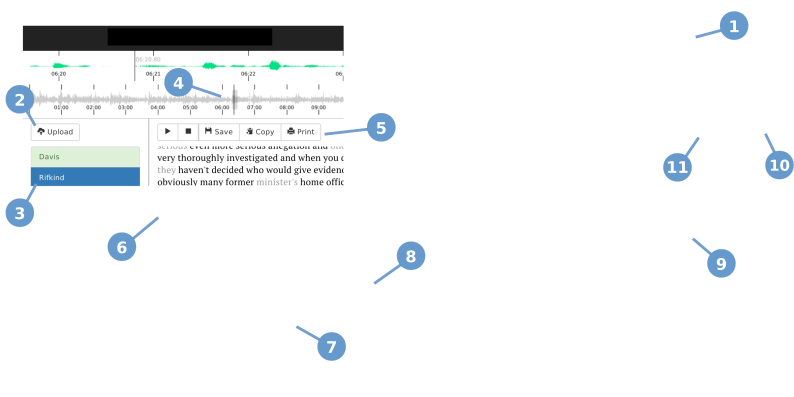
\includegraphics[width=\textwidth]{figs/interface-labels}
  \caption[User interface of Dialogger.]{User interface of Dialogger, with highlighted
    features: (1) individual user accounts and projects, (2) upload of audio recordings, (3) list of uploaded
    recordings, (4) waveform display of currently selected recording, (5) toolbar with playback, save, copy and print
    functionality, (6) transcript of selected recording with speaker labelling and word editing, (7) confidence
  shading, (8) transcript selection with drag-and-drop editing, (9) listing and re-ordering of edits, (10) duration of
edit, (11) export edit to audio file or digital audio workstation.}
  \label{fig:interface}
\end{figure}

\subsubsection{Transcript}\label{sec:transcript}

The ASR system we chose was evaluated using a large multi-genre television dataset \citep{Bell2015}.  It had an overall
word error rate of 47\%, however for news content, which is clearly spoken by a native speaker, this dropped to 16\%.
As the speech on radio programmes is similar in nature to speech on television news, we found the error rate to be
comparable. However, recordings with non-native speakers or significant background noise had a higher error rate.  For
comparison, the reported error rate of the system used by \citet{Whittaker2004} was 28\%, and for \citet{Sivaraman2016}
it was 10\%.

The time taken by the transcription service to process each uploaded recording was approximately half as long as the
length of the recording. The time depends primarily on the length of the recording but also on noise, accents and the
complexity of the speech.






\subsubsection{Operation}

The functionality and operation of the system is described below as a typical user journey. Each feature is numbered
and shown in Figure~\ref{fig:interface}.

Users access Dialogger by navigating to a web page in their browser. They start by logging into the system using their
account (1) and create a project where they can upload their speech recordings (2) that appear in a list on the left
(3). Each recording is automatically transcribed. When it is opened, the waveform appears at the top and the transcript
appears in the middle section.  The recording can be played (5) and navigated by using the waveform (4) or by clicking
on a word in the transcript (6). The transcript shows where different people are speaking using paragraphs labelled
with the speaker's gender and an identification number (e.g. [F2]). Words which are likely to be incorrect are shaded
grey (7), known as ``confidence shading''.  Incorrect words can be fixed by double-clicking them and typing the correct
word.  The transcript text can be copied or printed using buttons at the top. The audio can be edited by selecting a
range of words (8), then using drag-and-drop to place it in the area to the right which creates a clip (9).  Clips can
be re-ordered and deleted. The total duration of the edited clips is displayed (10). The edited audio can be played
through to preview the result, and the edit can be saved. Finally, the edited clips can be exported as a WAVE audio
file or as an EDL (11) for further editing in a DAW.



















\section{Evaluation methodology}\label{sec:screen-methods}

We wanted to determine whether professional radio producers could successfully employ the features of Dialogger as part
of the production of a real radio programme. Specifically, we were interested in measuring whether semantic speech
editing was faster than their existing technique, and if it continued to be used after the trial.  We also wanted to
investigate how the semantic editor was used and whether there were any features that could be added to improve the
functionality.

Additionally, we wanted to take this opportunity to continue our research on the existing radio production workflow to
learn more about the challenges producers face and the tools they use to produce their programmes. Our study in
Chapter~\ref{sec:ethno} did not explore requirements in-depth, and there is not much previous literature that analyses
actual radio production practice, so we wanted to be able to inform researchers and designers about real requirements
and behaviour in this field.

To achieve these goals, we conducted a qualitative contextual study of radio producers working under two conditions --
the existing editing workflow and the semantic editing workflow.


\subsection{Approach}
Gaining access to radio producers can be difficult as there are not many of them and they are normally very busy.
For example, \citet{Kim2003} attempted to recruit radio producers but was unsuccessful because the producers were ``so
highly tasked''. However, in this case we were able to recruit professional radio producers from the BBC Radio due to
the access available to us from working within the BBC.

As we would not be able to recruit a large number of participants, we chose to take a qualitative approach to maximise
the depth of the information gathering. To take advantage of the available access to the work environment, we chose to
use contextual inquiry techniques to allow us to learn about the workflows, tools, and the social, technical and
physical environments. This took the form of an initial interview, followed by a period of observation, then a final
interview.

Radio producers find it difficult to step away from their day-to-day work for too long.  To account for this, we
designed our study so that the tasks overlapped with
the production of the programme that the participant was working on at the time, and the audio
content they needed to edit that day. We interviewed and observed participants in their normal working environment to
ensure that the production workflow was not affected by an artificial setting.

\subsection{Recruitment}

We invited professional radio producers with at least five years of experience to take part by sending an email to
departments in BBC Radio that create pre-produced factual programmes.  Drama programmes were excluded from the study as
we saw in Chapter~\ref{sec:ethno} that their production workflow involves making multiple recordings of lines in a
script and selecting the best ones. This is a sufficiently different process to other programme genres that it warrants
a different interface.

Five participants (P1--P5) were recruited (4 male, 1 female) who each had between 6 and 20 years experience working
as a radio producer. Although we had a small number of participants, the experience of the producers and the depth of
the study means that their feedback should carry significant weight. Five participants is also considered sufficient
for identifying most usability problems \citep{Nielsen1993}.

During the experiment, the participants worked on programmes of different
lengths from a range of genres:
P1 produced a single 27-min documentary, %
P2 produced a 27-min documentary as part of a ten-part series,
P3 produced a single 45-min documentary,
P4 produced a 14-min archive programme
(based around material from the archive) as part of a ten-part series, and
P5 produced a single 27-min magazine show (covering multiple stories on a
single theme).

\subsection{Procedure}
We designed a five-stage experimental procedure that followed a typical contextual inquiry format of
interview/observation/interview. In addition, we recorded some simple metrics such as task completion time and feature
usage.

\paragraph{Stage 1: Background interview}
    The participant was first given an overview of the project and the study, and asked to complete a consent form. This
    was immediately followed by a semi-structured interview to learn about the participant's background, their existing
    production workflow and the tools they used. The investigator asked the participant to describe the
    radio production process in detail, and used follow-up questions to clarify their understanding. This information
    was recorded using written notes.

\paragraph{Stage 2: Dialogger training}
    Each participant was trained on the functionality of the Dialogger interface using a pre-written ``tool-tip tour'',
    in which the participant was presented with a sequence of instructional pop-up dialog boxes overlaid on the
    interface.  This ensured consistency of training between participants. Each participant was then issued with a
    series of tasks that utilised all of the system functionality. The investigator observed this stage and wrote notes
    of any unexpected behaviour or stumbling blocks.

\paragraph{Stage 3: Task observation}
    Each programme is composed of a number of interviews
    on a single topic, or set of topics.  We observed the participant while they logged and rough-edited two
    different interviews for the same programme. They did this by editing an interview under each condition -- one
    using their existing production workflow, and the other using Dialogger. The order of the conditions was
    counterbalanced.

    The investigator sat beside the participant during the task and wrote notes on the workflow, tools, generated
    metadata, usability issues, task completion time, and unexpected reactions or usage.
    The actions of the participant on Dialogger were logged electronically. After they completed the task, they were
    asked to rate each condition using the NASA Task Load Index metrics \citep{Hart1988}.


\paragraph{Stage 4: Interview}
    We conducted a semi-structured interview about the participant's experience of each system and how they compared.
    The investigator questioned participants about the advantages and disadvantages of each workflow, then asked about
    any specific topics, issues or questions that arose during observation. The audio from this interview was
    recorded and transcribed to allow for further detailed analysis.


\paragraph{Stage 5: Longitudinal deployment}
    Each participant was then given access to Dialogger for a further month, and was invited to continue to use it if
    they wished. Each week, they were asked via email whether they had been using the system, and if so, which features
    they valued most/least or were missing.  During this time, their usage of Dialogger was also logged electronically.

\subsection{Analysis}
Our study produced observation notes, interview transcripts and metrics. We used thematic analysis with open, flat
coding to interpret the textual data, and we used statistical analysis to process the numerical data, as described below.

\subsubsection{Coding}
We manually transcribed the audio recorded from the interviews in Stage 4 to produce a verbatim transcript, and
collated them with notes made by the investigator from stages 1, 2 and 3. To organise and process this textual
information, we employed the use of thematic analysis \citep{Braun2006}.

We performed a two-stage coding process.  Firstly, we openly coded each part of the transcripts
into a flat structure.  As there are not many previous studies on radio production, we decided to
use open coding so that the categories would emerge from the data we collected, rather than attempting to test an
existing model.  We used the software package RQDA \citep{RQDA} to execute this stage.

Once all of the text had been processed, we grouped the codes that had common themes. We used mind-mapping software to
help us re-arrange the codes into various hierarchical structures until a logical solution was found.  The coding
and grouping was performed by the investigator that collected the data.

\subsubsection{Metrics}
Although this was primarily a qualitative study, we chose to collect some basic metrics to measure task completion
time, cognitive load and usage after the trial.

We used task completion time from Stage 3 as a metric for editing speed. As participants used different interviews of
varying lengths for each condition, we measured task completion time relative to the length of the audio
recording being edited. We used a paired \textit{t}-test \citep[p.~17]{Shalabh2009} to test for any significant
difference between the existing and semantic editing workflows.

To measure the cognitive load of each task, we used the raw TLX metrics gathered from the questionnaire in Stage 3. We
used a paired \textit{t}-test on each of the six metrics to test them individually for any significant differences.

Finally, to measure the level of usage during the longitudinal deployment in Stage 5, we collected the time spent using the
interface, the number of new uploads and the number of exported edits. As this data is only relevant to the semantic
editing workflow, we will report the raw numbers.

\section{Results}\label{sec:screen-results}

The coding process resulted in 40 codes, which were grouped into ten categories and four themes (see
Table~\ref{tab:codes}). The codes contain comments about both the existing and semantic editing workflows, however for
clarity we will present these results individually.

We start by going through the existing radio production workflow in detail, with an emphasis on the challenges that
were identified, and the tools that are used as part of the process. We then consider the semantic editing workflow and
expand on the four themes identified during coding. Finally, we look at the results of the metrics that we captured
during the observation and longitudinal deployment.

\begin{table}[h]
\centering
{\small
\begin{tabular}{p{0.18\linewidth} p{0.2\linewidth} p{0.5\linewidth}}
\hline
\textbf{Theme} & \textbf{Category} & \textbf{Codes} \\ \hline
\multirow{5}{*}{Comprehension}
 & Challenges & Complexity, quantity, environment, concentration, time taken \\ \cline{2-3}
 & Navigation & Speed, search, paragraphs, speaker segmentation, time since recording, cross-referencing \\ \cline{2-3} 
 & Accuracy & Correction, accents, good enough, confidence shading, use after editing \\ \hline 
\multirow{3}{*}{Organisation}
 & Mark-up & Bold, star rating, labelling, annotation, timestamps, word processing \\ \cline{2-3} 
 & Programme script & Structuring, collaborating with presenter \\ \hline 
\multirow{2}{*}{Editing}
 & Sound quality & Fast playback, anxiety of not listening \\ \cline{2-3}
 & Technique & Deleting, workflow, transcript not needed for short edits, similarity to TV \\ \hline
\multirow{3}{*}{Usability}
 & Portability & Laptop, paper \\ \cline{2-3} 
 & Drag'n'drop & Space on clipboard, scrolling \\ \cline{2-3} 
 & Misc & DAW integration, transcript turnaround time, simultaneous uploads, video support, waveform, avoidance of repetition \\ \hline
\end{tabular}
}
\caption{Topics, categories and codes that emerged from analysis of the interviews in Stage 4 and the
observation notes from Stages 1, 2 and 3.}
\label{tab:codes}
\end{table}

\subsection{Existing workflow}\label{sec:resultsexisting}



In this section, we consider the comments made by participants about their existing workflow. We have organised these
by the categories from the thematic coding (see Table~\ref{tab:codes}).
























\subsubsection{Challenges of comprehension}

The skill of the producer is to \textit{``separate the wheat from the chaff''} (P1, P3, P4 -- all verbatim) and to find
the clips which will make an interesting programme.

\textit{``That's the basis of my job - to find great stuff and put it together.
  It's not difficult putting it together, it's finding the great stuff and finding connections between it. Getting rid
  of the non-great stuff is
  challenging and time-consuming, and it requires mental processing.''} (P1)

However, the sheer quantity of recordings means this process adds significant overhead.

\textit{``you've got an average of 45 mins per interview and in a series of
  three programmes you've got seven per programme, that's a lot of work''} (P3)

Interviews recorded for speech radio often cover complex topics in fine
detail. Keeping track of all the points raised and forming a compelling
narrative from them is a challenge.

\textit{``All the interviews overlap with each other terribly, and have got
  similar themes.''} (P4)

Writing the logs takes a lot of concentration as the producer must listen to
what is being said, work out how it ties in with other contributions and the
story, and make swift judgements on whether it should be used.

\textit{``one of the slightly exhausting things about doing it is the level of
  concentration you have to maintain to make good decisions, remember where
  everything is, what you've got, is kind of strained rather by having to just
  do schleppy tasks like moving the sound and logging interviews''} (P3)

P1 and P5 reported that they find the office environment distracting, so often work at home or outside the office.

\textit{``I typically do this at home because I find it a much less distracting
  environment. It does require quite intensive concentration so you don't miss
  something.''} (P1)

\textit{``In the office there's so much pressure and you're always doing stuff.''} (P5)

Although P4 did not do any logging during observation, they explained that for longer recordings, they
would normally write logs by hand in a notebook whilst listening on a
portable music player somewhere away from the desk, such as in a caf\'e.

The high level of concentration required, combined with the repetition of 
typing and listening to the interview again means that producers need to take
regular breaks.

\textit{``it's boring and it's not very easy to be efficient at it [...] when
  I'm normally doing it I'm checking my emails, making a cup of tea.''} (P3)

\subsubsection{Programme script}
The producers organised the programme by writing a script. This is primarily used to help them structure their
thoughts, but also to help communicate with the presenter over email.

In the study, P1, P2 and P5 started their scripts during the research stage by writing an ordered list of bullet points
of topics to cover and a list of draft questions to ask contributors.  P3 and P4 waited until after they had done some
interviews to start the script, as they wanted to structure the programme around the discussions that they recorded.

P3 and P5 updated the script after every edit to ensure they were always in sync. This added significant overhead but
gave them a visual structure to follow when making the final changes.
Having an accurate script also makes it easier to re-use the programme afterwards, when creating another version of a
different length, or for pulling out clips for the website.

\textit{``[The script] is going to be invaluable when it comes to re-cutting this.''} (P5)

\subsubsection{Mark-up}

P1, P3 and P5 would make comments for themselves in the log to help them when
editing. For example, ``\textit{[good to here, dull after]}'' or
``\textit{[trails off 9'30]}''. P1 also used a star rating system to rate the
quality of each point, for example ``\textit{[**** should use this stuff, but
  dramatically cut down]}''.

\textit{``What I sometimes do when I edit is star good bits, and I think
  that's quite a common trait.''} (P3)

Bold highlighting was also used by P1 and P3 to mark bits of the transcript
which are important and worth keeping.

\textit{``what I did was just put in bold the paragraphs I thought were worth
  [keeping]''} (P1)

P2 used a different approach to logging their material. Instead of logging the material by writing a transcript, they
played the recording in a DAW and used a keyboard shortcut to create timed markers at any points of interest. By seeing
where the markers clustered, they identified where to make clips, then gave each of the clips labels. This approach
allowed them to focus more on the audio, but didn't allow them to make any detailed notes.

\subsubsection{Sound quality}\label{sec:existing-quality}

Radio is an audio-only medium, so the quality of the content is highly dependent on the quality of the sound.  The
criteria producers use for deciding whether a piece of audio is good enough to use in their programme is not just about
what was said, but how it was said and how well it was said.

\textit{``How people say things is very important.''} (P5)

On the one hand, producers need to listen out for any poor quality sound that might negatively affect the programme,
such as people mumbling, stumbling, coughing, or any excessive background noise. 

\textit{``I've done paper edits before where I've gone back to that bit of audio and they didn't quite finish the
  sentence or they muttered it. You just couldn't use it at that point.''} (P3)

However, the producers were also listening out for anything that worked particularly well, such as a moment of
comedy or passion, or a sound that perfectly captures the right feeling. Identifying these using the text of a
transcript is very difficult or impossible. 

Every participant that performed logging played the audio faster than real time at least once. This allowed them to
efficiently listen out for anything they might want to use while reviewing parts of the interview that may not be of
interest (e.g. off-topic or ``off-mic'' discussions).  P2 also used faster playback to prevent themselves from
over-thinking their edit decisions and picking out too much material.

\textit{``The ability to listen at faster than real-time [...] gives me the opportunity to come to a swifter decision.''}
(P2)


\subsubsection{Edit technique}

If the recording was short and had been recorded recently, as was the case for P4 and P5, it can be edited
without first creating a log.

\textit{``If it's a quick ten minutes with three questions, you don't need to bother''} (P3, also P4 and P5)

In this situation, we observed that the producers listened through the recording using a
DAW and pressed a keyboard shortcut to split the recording, usually at the beginning/end of questions/answers. They
then went back to remove unwanted segments and add labels to the remaining ones.

In the cases where the recording was logged (P1, P2, P3), the producers used the log to decide which parts to select or
remove. They used the timestamps written in the log to narrow down their search area for each clip they extracted.
However, even with a reduced search area, the producers found it time-consuming to find the exact start and end point
of each clip using the DAW interface.

In the study, three of the participants (P3, P4 and P5) used SADiE as their DAW, which is provided to the producers by
the BBC. However, the other two participants chose to use other software packages that aren't formally supported. P1
used Adobe Audition because they were familiar with the interface and it was installed on their laptop, unlike SADiE
which was only available to them on a desktop computer.

P2 comes from a television production background and used Apple's Final Cut Pro, which is primarily a video editor but
also includes audio editing functionality.  P2 used Final Cut Pro because they were familiar with the interface and had
it on their laptop. In addition, they enjoyed being able to import audio directly from video content without having to
use another program to extract the audio first, and being able to use the video ``titles'' feature to make written notes
that can later be viewed in time with the audio.

\subsection{Semantic editing workflow}\label{sec:resultsnew}
This section discusses the results and themes that emerged from the evaluation of the semantic editing interface.
Participants were first introduced to Dialogger through a training stage (Stage 2). All of the
participants completed the training without any major issues. However, this stage highlighted a requirement for
keyboard shortcuts which was not previously identified.  P2 and P3 kept trying to use the space bar to start and pause
audio playback. This is a common shortcut in most DAWs which these participants naturally reached for. Reports on
previous semantic editing systems have not mentioned keyboard shortcuts, however they could be used to assist the
editing process.

In the rest of this section, we will discuss each of the themes that came out of the thematic coding (see Table~\ref{tab:codes}).












\subsubsection{Navigation}

Participants reported that having the transcript available in the semantic
editing interface allowed them to read and search the recordings much faster
than they normally would with a waveform, which is in line with previous findings from
\citet{Whittaker2004} and \citet{Yoon2014}.

\textit{``with having a transcript you're able to immediately scan through it
  10/15 times faster. Maybe that's an exaggeration but it feels ten times
  faster''} (P1)

The transcripts also allowed the participants to quickly cross reference what
was said in various interviews without having to listen through multiple times.

\textit{``where I'm picking shorter clips, making a point and moving on or I'm
  developing an argument between different people and cutting between them, it
  feels a lot more easy to construct that `on paper' than what I'm currently
  doing''} (P2)


Being able to click on a word to navigate to that point in the audio also
enabled the participants to use visual search to quickly find and listen to
bits they were looking for.

\textit{``you can do that with your eyes even quicker - zone straight in on the bits and that click to go  `that bit',
  `that sentence there', `that word there' ''} (P4)

Participants reported that editing with a transcript was primarily useful when working at the sentence level. When the
granularity of editing involves removing individual words, ``umm''s or breaths, they said that the DAW software is much
better suited to these tasks. This supports our design decision to integrate with DAWs.

\textit{``the real editing work actually happens after this has passed its main
  point of usefulness''} (P3)









\subsubsection{Transcript accuracy}
When using the semantic editing interface, editing decisions are based on an
automated transcript which is only partially accurate. Previous research has shown that for editing
voicemail recordings \citep{Whittaker2004}, discussions \citep{Sivaraman2016} and spoken comments \citep{Yoon2014},
automated transcripts were considered sufficiently accurate. However, the ASR transcript accuracy required for
navigation and editing in radio production is currently unknown.

The participants in our study suggested that the transcripts were, generally speaking, sufficiently accurate for their
purposes.

\textit{``It's clearly not 100\% in word recognition but I'm feeling it's
  certainly good enough for my rough cut purposes at this point''} (P2)

If the recording being edited was made recently, the producer can use their
memory of what was said to make sense of the inaccuracies in the
transcript.

\textit{``Both these interviews [being edited] are relatively recent so I have
  it reasonably in my mind what they've been saying. I was able to read roughly
  what there was - `okay that's that question', `I know what was in that
  question' ''} (P1)

In the existing radio production process, transcripts are used to aid the producer and presenter, but are
  not shared outside of the production team. In our study, the producers we observed only used the transcript
  to navigate and edit the audio. However, P3 and P4 noted that they were interested in correcting the transcript later
  so it could be shared or published.

\textit{``I'm probably posting transcripts for the whole interview. So I do
  need to go through and correct''} (P4)

Being able to provide corrected transcripts has the potential to make an impact beyond improving the
  editing workflow. For example, transcripts of the finished programme could make the audio content searchable and
  re-usable for print media.















\subsubsection{Mark-up}



During the study, P1 and P3 copied the transcript text from the interface into Microsoft Word. They
reported that they did this because there was no annotation functionality
available within Dialogger.

They inserted paragraph breaks, added notes after paragraphs, and
highlighted desired parts of the transcript in bold. Once the transcript was
annotated in Microsoft Word, they went back to Dialogger, found the parts of the
transcript they wanted by scrolling though the text, then dragged and
exported each clip individually as a WAVE file.

\textit{``it would be better to take raw lumps of transcripts and plonking them
  in Word because Word has higher functionality than this''} (P3)

Producers are very familiar with the Microsoft Word interface so a later version of our
system could seek to provide a similar interface. This would allow producers to make annotations in the same way they
do already.

\textit{``With text editing, the reflexes are very much Microsoft Word''} (P4)

The most basic feature that could be added is highlighting, which is often used to note parts of interest

\textit{``If you just put a little star or underline or something simple to
  mark things, that would be a big gain for a small change''} (P3)




\begin{figure}
\centering
  \includegraphics[width=\columnwidth]{figs/print/highlighting-cropped.jpg}
  \caption{Printed transcript that has been highlighted by P2.}
  \label{fig:highlight}
\end{figure}

\subsubsection{Portability}

P5 reported that working on paper allowed them to be productive outside of
the office, such as during their commute.

\textit{``What would be really useful would be to [...] take it away (say when
  I'm on the train going home) and I would paper edit the bits that I need''}
(P5)

Additionally, working on paper allows them to work anywhere as it does not
require electricity.

\textit{``It's highly portable. It doesn't require any power.''} (P2)

In the observed task, after uploading their recording, P2 immediately printed
the transcript and read through it on paper so that they could work away from
the screen.

\textit{``I'm reading a lot of material for a sustained period so I'd prefer to do it on page than on screen. Just
  easier on my eyes.''} (P2)


P2 then used a highlighter pen to select the desired parts of the recordings (see Figure~\ref{fig:highlight}).  After
highlighting all the pieces they wanted,
they then used the Ctrl+F text search to find the highlighted words in Dialogger.

\textit{``it allowed me to get to clips very quickly from a reference point on a printed transcript''} (P2)

However, P2 noted that having timestamps on the printout may be a faster
way of achieving the same thing.
Once they had found and clipped all of the highlighted parts in Dialogger, they exported the clips into SADiE.

P4 explained that for an upcoming programme, they were
planning to print out transcripts from Dialogger to help
them collaborate with their presenter.

\textit{``we're just going to go through it with a pencil and paper, with a
  printout, and highlight the bits we want and cross out the bits we don't.''}
(P4)

\subsubsection{Sound quality}
Part of the appeal of having a transcript is that it frees the user from listening to the audio in real-time. It also
allows users to work on paper, away from any electronic devices. However, disconnecting the audio from the text
fundamentally changes the production process.

\textit{``Radio is made with your ears. You'll never get away from that fact that you need to listen''} (P4, also P2,
P3, P5)

There was also concern that parts which sounded great but didn't come across as well in the transcript may have been
overlooked.

\textit{``I was anxious it might not have sounded as good as it read, or that I might be missing bits that sounded
  great ''} (P2)

As discussed in Section~\ref{sec:existing-quality}, the existing workflow of the participants includes playing the
audio faster than real time, but that feature was not included in Dialogger.  Several of the participants noted that
they would like to have this feature added.

\textit{``it's a little bit annoying that there's no facility for that.''} (P2)

Although faster than real time playback normally reduces intelligibility, this may be less of a problem if the
transcript was available.

\textit{``you do still need to listen through, even though you've got the text.  Therefore, it would be optimised if we
  could listen through quickly''} (P4)

As listening is an important part of the production process, semantic audio interfaces would benefit from providing
easy access to the underlying audio to allow multi-modal interaction. Once the link between the audio and the text is
broken, re-linking the two together can be costly.



\subsubsection{Drag-and-drop}

In Dialogger, we used a drag-and-drop technique for users to create clips from various interviews and
re-order them in a clipboard area. All of the participants were able to use this successfully, however we quickly
encountered issues when dealing with longer clips.

\textit{``I found the interface quite clunky for pulling out big chunks of audio''} (P5)

We performed our initial testing by pulling short clips, but for real-life usage, participants were mainly interested
in creating large clips. This quickly filled up the clipboard area and users struggled to find the space to add more
clips. This finding is in contrast to \citet{Sivaraman2016} which found that participants were mainly interested in
making small edits.

P2 suggested modifying the interface so that clips were created by selecting the text and using a button to add the
clip to the end of the clipboard. The problem could also be addressed by collapsing and expanding the clips to minimise
the area they occupy.


\subsubsection{Usability}

Users could transfer their edits from Dialogger to a DAW by saving and opening a file. However, some
participants wanted much tighter integration with the DAW, including bi-directional transfer of edits, so that edits
made in the DAW were reflected in the semantic editor and vice-versa.

\textit{``Instead of thinking about it as a paper edit, if you think of it as the paper edit result of the sound
  edit''} (P3)

None of the participants found the waveform display in Dialogger to be useful, and found it to be an
unnecessary addition to the transcript text.

\textit{``You're either working with text or working with the waveform. You don't need both.''} (P5)

Some participants also noted that they would prefer a cut-and-paste approach to copy-and-paste, as this prevents any
duplication of content. This could also be achieved by marking which parts of recordings have already been used.

\textit{``When you have a big load of stuff, it's comforting to know that you're not duplicating your work.''} (P4)

































\subsection{Metrics}\label{sec:resultsmetrics}
\subsubsection{Time}

\begin{figure}
\centering
  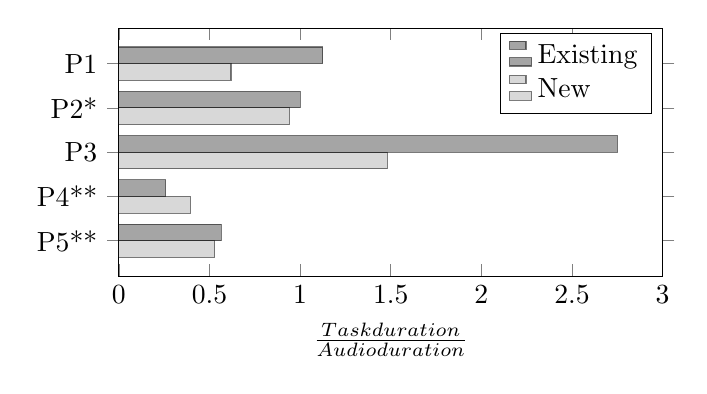
\begin{tikzpicture}
  \begin{axis}[
      width=.7\columnwidth,
      xbar=0pt,
      bar width=6pt,
      xlabel=$\frac{\text{Task duration}}{\text{Audio duration}}$,
      y=16pt,
      xmin=0,
      xmax=3,
      enlarge y limits=0.2,
      symbolic y coords={P1,P2*,P3,P4**,P5**},
      ytick = data,
      y dir=reverse,
      reverse legend,
      legend cell align={left},
      ]
  \addplot[fill=black!30, opacity=0.5] coordinates {(0.619,P1) (0.941,P2*) (1.48,P3) (0.395,P4**) (0.529,P5**)};
  \addlegendentry{New}
  \addplot[fill=black!70, opacity=0.5] coordinates {(1.125,P1) (1.0,P2*) (2.75,P3) (0.258,P4**)
    (0.565,P5**)};
  \addlegendentry{Existing}
  \end{axis}
  \end{tikzpicture}
  \caption[Time taken to complete the task for each condition, compared to the original audio length.]{Time
  taken to complete the task for each condition, compared to the original audio length. Lower is better. *P2
  logged their material on paper. **P4 and P5 did not do any logging. Due to the small sample size and variation in
  usage, no conclusions about time performance can be drawn.}
  \label{fig:time} \end{figure}

We recorded the time participants took to complete the observed tasks (see Figure~\ref{fig:time}). As various
recordings of different lengths were used for the existing and new workflows, we divided the edit time by the audio
duration to calculate the relative edit time.  In all cases, the producers were able to run the ASR processing as a
background task so this was not included in the calculation. P1, P2 and P3 used the semantic editor after their
existing process, while P4 and P5 did the opposite. However, as different recordings were edited on each system, the
presentation order is not expected to affect the results.

The mean average time for semantic editing was 0.79 minutes per minute of audio, versus 1.13 minutes for the existing
method, which is a 44\% improvement. However, a paired \textit{t}-test revealed that there was no statistically
significant difference (\textit{p} = 0.24).  This is due to the small sample size and the large variations in timings
resulting from P4 and P5 not doing any logging, and P2 printing out and annotating their transcript before editing.
Semantic speech editing may have the potential to reduce the time needed for logging and rough-editing material, but
further investigation with a larger sample and consistent workflow is required to measure time performance.




\subsubsection{Cognitive load}



After completing both tasks in the observation, the participants were asked to
rate both the old and new workflows using the raw NASA-TLX metrics
\citep{Hart1988}.
No significant differences were detected for any of the metrics using the paired \textit{t}-test.
With only five participants and marginal differences, it was not possible to
draw any conclusions about cognitive load from these results.  They indicate
that Dialogger requires slightly less effort and mental demand, and is less
frustrating.
However, it is considered more physically demanding, temporally
demanding and scores lower in performance.



\subsection{Longitudinal deployment}

After the interviews and observations were complete, the participants were given access to Dialogger for a further
month (Stage 5). During this time their actions were logged electronically and they were emailed each week to ask which
features they found useful, or were missing. P3 was unavailable immediately after the study, so could not take part in
this stage.

Most of the comments received in the longitudinal deployment were already picked up by the first part of the study. In
the remaining comments, all of the participants said they enjoyed being able to use Dialogger outside of the office and
at home. Some reported that they had issues uploading content with their slow network connections, and P2 suggested
that allowing multiple simultaneous uploads would allow them to leave it running overnight.

Participants were given access to the system for one month after the study.  The logs from the interface were analysed
to see how the participants used Dialogger during this stage of the study.
All of the participants continued to use the semantic editor of their own accord as part of their work. The total time
spent by the four remaining participants (P1, P2, P4, P5) using Dialogger in the month-long deployment period was 23
hours and 58 minutes.  Over 14 hours of those were from P2, with P4 using it for 5 hours, P1 for 3 hours and P5 for 20
minutes.  During this period, 86 recordings were uploaded and 58 audio edits were exported.


Users could navigate the content by either clicking on the waveform or by clicking on a word in the transcript. The
interaction log showed that over 98\% of navigation actions were executed by clicking on a word, which shows a clear
preference for navigating by text compared to waveforms.





\section{Discussion}\label{sec:screen-discussion}
We found that producers face a number of challenges with audio editing in radio production. There is often a large
quantity of audio to process so it can take a long time. The content of the speech is usually complex and contains
interconnections to things said in other recordings, which can be difficult to keep track of. Making editorial
decisions also requires a high degree of concentration over an extended period, which is demanding, especially in the
noisy and distracting office environment.

We observed that in their existing workflow, participants tackled these challenges by employing a number of techniques
to filter and arrange their audio content. They started by listening back to all of their recordings, which allowed
them to simultaneously assess the editorial content and sound quality of the audio. For long recordings, many
participants \textit{logged} the audio as they listened, by typing rough transcriptions and notes into a word processor, which
they later used to help them edit the audio using a digital audio workstation (DAW). For short recordings, instead of
logging, participants segmented their recordings in the audio editor during playback, and went back to remove unwanted
segments and label the rest.
All of the participants used a word processor to create a programme script in which they developed the structure and
content of their story. They used annotations to highlight or rate the transcripts, and wrote notes to help them with
selecting and assembling the final content.

We introduced a semantic editing system into professional radio production, which the study participants were able to
successfully use as part of their workflow. On average, the semantic editing workflow was much faster than the existing
workflow, in line with previous findings from \citet{Whittaker2004}, but this result was not statistically significant,
so requires further investigation.  We compared the semantic editing workflow, which included a transcript, to the
existing workflow, which did not. Therefore, we were unable to measure how much benefit was derived from the transcript
itself, compared to the semantic editing interface.  All participants voluntarily continued to use the system after the
trial, which indicates that they found value in using it. However, we identified a number of important features that
were missing or could be used to improve future semantic speech editing systems. These related to listening,
annotation, collaboration and portability.

\subsection{Listening}

Logging is an important process that primarily involves labelling and organising content, however it is time consuming.
Some participants found the logging process to be valuable
because it gave them the opportunity to listen back through their recordings, and make connections between various bits
of content. This cross-referencing could also be assisted by providing links between words within and between
recordings. For example, selecting a word could display and replay other mentions of that word in other recordings.

Another important reason for listening is to ensure a high ``sound quality''. Participants wanted to avoid low quality
audio such as ``umm''s, mumbling, coughing and excessive background noise, but they also wanted to ensure they didn't
miss any high quality audio moments that might not have been identified using the transcript.  Faster playback is
already used in radio production to reduce the time spent listening to material, however more sophisticated time
compression algorithms such as those described by \citet{Arons1997} could be used. Time compression has not been
included in previous semantic editing systems, but should be considered in the future, especially as \citet{Vemuri2004}
found that the maximum time compression factor is significantly higher when an automated transcript is present.

Removal of ``umm''s and breaths through de-umming is either done by the producer themselves or with the help of a sound
engineer, depending on the producer's experience and time pressure. To maintain sound quality, the removal of
umms/breaths must be audibly transparent and participants reported that this can be difficult to achieve.  Previous
semantic editing systems have included functionality to remove umms \citep{Berthouzoz2012} and breaths
\citep{Rubin2013}, however these were made possible because the manually generated transcripts explicitly transcribed
those items. ASR systems are normally trained to ignore umms/breaths rather than transcribe them, which prevented us
from including this functionality. A transcription system that includes these would allow us to add this functionality,
however further research is needed into the extent to which de-umming can be automated in this way.

\subsection{Annotation}

All of the participants used a script document to structure and assemble their programme, and as a
medium to inform and gather feedback from the presenter about the content and layout of the programme. Although the
clipboard of our semantic editing system acted much like a programme script, the participants did not use it in that
way because it was missing some key functionality for annotation and collaboration.

Annotation features were an important requirement that we did not pick up on during the design specification, and which
have not been included in previous semantic speech editing systems. Two participants in our study deviated from the
expected workflow in order to annotate the transcript, and the other participants noted the absence of such
functionality. Participants wanted to be able to annotate the transcripts as they would with a word processor, in order
to highlight or rate particularly good parts of their recordings, add personal comments, and to segment and label the
content.

A simple change to achieving this would be to allow the transcripts to be formatted, and for textual comments to be
inserted and edited. Furthermore, the drag-and-drop editing could be replaced with cut/copy/paste similar to
\citet{Whittaker2004} and \citet{Rubin2013}. An alternative approach could be to add semantic speech editing
functionality to a word processor, rather than adding word processing functionality to a semantic speech editor.

\subsection{Collaboration}

Scripts are used as a tool for collaborating with colleagues such as the
presenter because the programme's content and structure can be quickly reviewed and
commented on by others without them having to spend time downloading and listening to the audio. Our semantic editing
system was designed for individual access to transcripts and edits, however this meant that they could not be shared
with the presenter. A better approach would be to allow multiple users to navigate and edit the same material. This
could be achieved using operational transformation \citep{Sun2004} which can support concurrent users editing the same
content. Participants were also interested in tighter integration with the DAW. The same technology could be used
to create bi-directional integration with DAWs, so that any edits made in the DAW are automatically updated in the
semantic editor and vice-versa.

\subsection{Portability}

Participants reported that the open-plan office environment in which they worked was often noisy and distracting, and
that they had difficultly working on screens for extended periods. As a result, many reported that they work from home
to get away from the office or print transcripts so they can get away from the screen. A more portable semantic speech
editing system would allow producers the flexibility to work where they wanted.

Digital pen interfaces such as the Anoto system could be used to create a paper-based semantic editor that can be used
anywhere and does not involve screens. Additionally, it naturally supports freehand annotation and may be a better
medium for face-to-face collaboration.  \citet{Klemmer2003} has previously explored how speech can be navigated using
paper transcripts and \citet{Weibel2008} describes how an Anoto system can be used to edit digital documents, however
these approaches have yet to be combined.

\subsection{ASR transcripts}

Participants reported that the automatically-generated transcripts were sufficiently accurate for editing, supporting
similar previous findings from \citet{Whittaker2004} and \citet{Sivaraman2016}. This is helped by the fact that radio
producers record the audio themselves, and can use their memory to cope with inaccuracies. Most participants were only
interested in correcting errors that were distractingly wrong, which were often names or locations related to the
story. However, as these are known ahead of time, they could be provided to the ASR system as a way to tweak
or expand the language model.

Currently transcripts of each programme are not published due to the high cost and
overhead, however several participants were interested in fully correcting their transcripts so they could do this.
The availability of ASR transcription could have the potential to extend the scope of radio production to include
publication of transcripts. This could help to improve discoverability of programme content, especially if word timings
were included.






















































\subsection{Outcome}
Based on the results of this work, we developed the prototype further to take into account the feedback from the
producers in our study.  We handed the prototype over to a development team at the BBC who turned it into an
officially supported production tool.  This has allowed producers from around the BBC to use the tool as part of their
normal workflow.  As of October 2016, the system had 45 active users and had processed 265 audio recordings.

\begin{figure}
\centering
  \includegraphics[width=.8\columnwidth]{figs/descript.png}
  \caption{User interface of the \textit{Descript} semantic speech editor, a commercial semantic speech editing system
  developed independently of our research.}
  \label{fig:descript}
\end{figure}

Independently of our research, in late 2017, a commercial semantic speech editing system called \textit{Descript} was
released\footnote{\url{https://www.descript.com/}}. Descript is an audio production interface that uses ASR and manual
transcription to allow users to transcribe and edit their audio. The interface, shown in Figure~\ref{fig:descript},
includes annotation features such as bold, italic, highlighting and time markers.  Rather than using a drag-and-drop
technique for editing the audio, Descript uses strikethrough annotation to remove segments of audio. The transcript can
be corrected by switching from editing mode to correction mode, and the transcript includes speaker diarization.  In
addition to these features, Descript includes an integrated waveform editor that can be used for fine editing and
inserting cross-fades.  This recent commercial interest in semantic speech editing suggests that there is interest in
using this technology for audio production, and that ASR systems are now sufficiently accurate to support it.














\section{Conclusion}\label{sec:screen-conclusion}
We conducted a contextual study of semantic speech editing in professional radio production. The participants were able
to use our system to produce real programmes and they continued to use it after the study.  However, the results
highlighted a number of opportunities to better address the needs of radio producers.
Annotation features such as highlighting, ratings and comments are needed to aid producers in organising and
structuring their content.
Radio production is a collaborative process, so semantic editing tools should support multiple users. Use of
operational transformation would allow concurrent editing and integration between multiple interfaces.
Some participants struggled with office and screen-based working so portable interfaces, such as those offered by
digital pen technology, would give producers the flexibility to work where they are most productive. 
Unwanted noises such as ``umm''s and breaths must be removed transparently, which is done by the producer or sound
engineer. By training ASR systems to transcribe these noises, this could be done in the semantic editor.
However, further research is required into the sound quality achieved by this approach.
Finally, ``radio is made with your ears'' so there are limits to how much editing can be done using a text-based
interface. Editing tools should provide easy access to playback and use time compression features, which allow users to
listen much faster, particularly in combination with the transcript.


